\subsection{Histograms}


\begin{lstlisting}
from sie import *
\end{lstlisting}

Load a sample data set, and select only the Male data...

\begin{lstlisting}
data=load_data('data/survey.csv')
male_data=data[data['Sex']=='Male']
\end{lstlisting}

select only the height data, and drop the missing data (na)...

\begin{lstlisting}
male_height=male_data['Height'].dropna()
\end{lstlisting}

make the histogram

\begin{lstlisting}
hist(male_height,bins=20)
xlabel('Height [cm]')
ylabel('Number of People')
\end{lstlisting}

\begin{verbatim}
<matplotlib.text.Text at 0x1085728d0>
\end{verbatim}

\begin{center}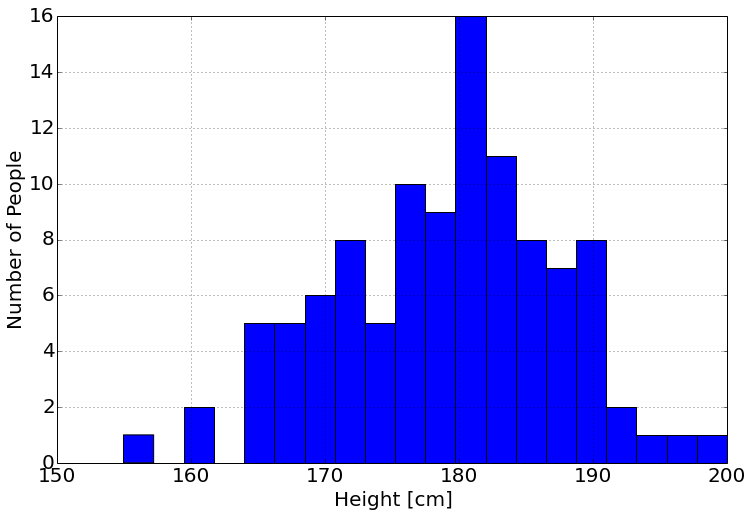
\includegraphics[width=4.5in]{Random_Sequences_and_Visualization/Random_Sequences_and_Visualization_fig0.png}\end{center}

\subsection{Scatter Plot}


\begin{lstlisting}
from sie import *
\end{lstlisting}

Load a sample data set, and select only the Male data...

\begin{lstlisting}
data=load_data('data/survey.csv')
male_data=data[data['Sex']=='Male']
\end{lstlisting}

select only the height and the width of writing hand data, and drop the missing
data (na)...

\begin{lstlisting}
subdata=male_data[['Height','Wr.Hnd']].dropna()
height=subdata['Height']
wr_hand=subdata['Wr.Hnd']
\end{lstlisting}

plot the data

\begin{lstlisting}
plot(height,wr_hand,'o')
ylabel('Writing Hand Span [cm]')
xlabel('Height [cm]')
\end{lstlisting}

\begin{verbatim}
<matplotlib.text.Text at 0x1085774d0>
\end{verbatim}

\begin{center}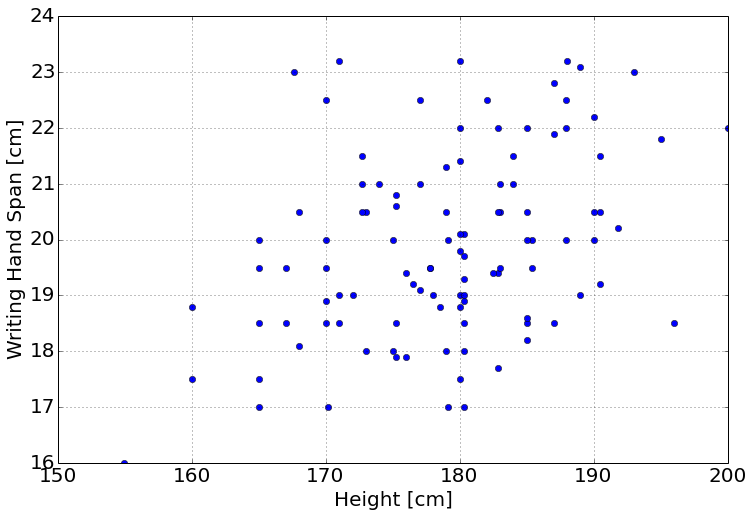
\includegraphics[width=4.5in]{Random_Sequences_and_Visualization/Random_Sequences_and_Visualization_fig1.png}\end{center}

